\chapter{Implementacja}
Aplikacje testowe miały za zadanie sprawdzać dostępność najczęściej wykorzystywanych mechanizmów używanych do budowy aplikacji internetowych. Aby rozwiązywały one rzeczywisty problem, miały one pełnić rolę aplikacji do zarządzania inteligentnym budynkiem. Tematyka ta nawiązuje do mojej pracy inżynierskiej, której tematem był ,,System zarządzania inteligentnym domem z wykorzystaniem Raspberry Pi oraz technologii internetowych''.

W każdej z aplikacji zostały zaimplementowane następujące funkcjonalności:
\begin{itemize}
  \item rejestracja i logowanie użytkowników - system autentykacji,
  \item dodawanie i usuwanie sensorów,
  \item dodawanie i usuwanie danych zbieranych przez sensory,
  \item przetwarzanie danych w tle na przykładzie przetwarzania plików CSV z danymi użytkowników.
\end{itemize}

Każda z aplikacji obsługuje bazę danych o strukturze, która przedstawiona jest na rysunku \ref{fig:diagram_erd}.

\begin{figure}[h]
  \centering
  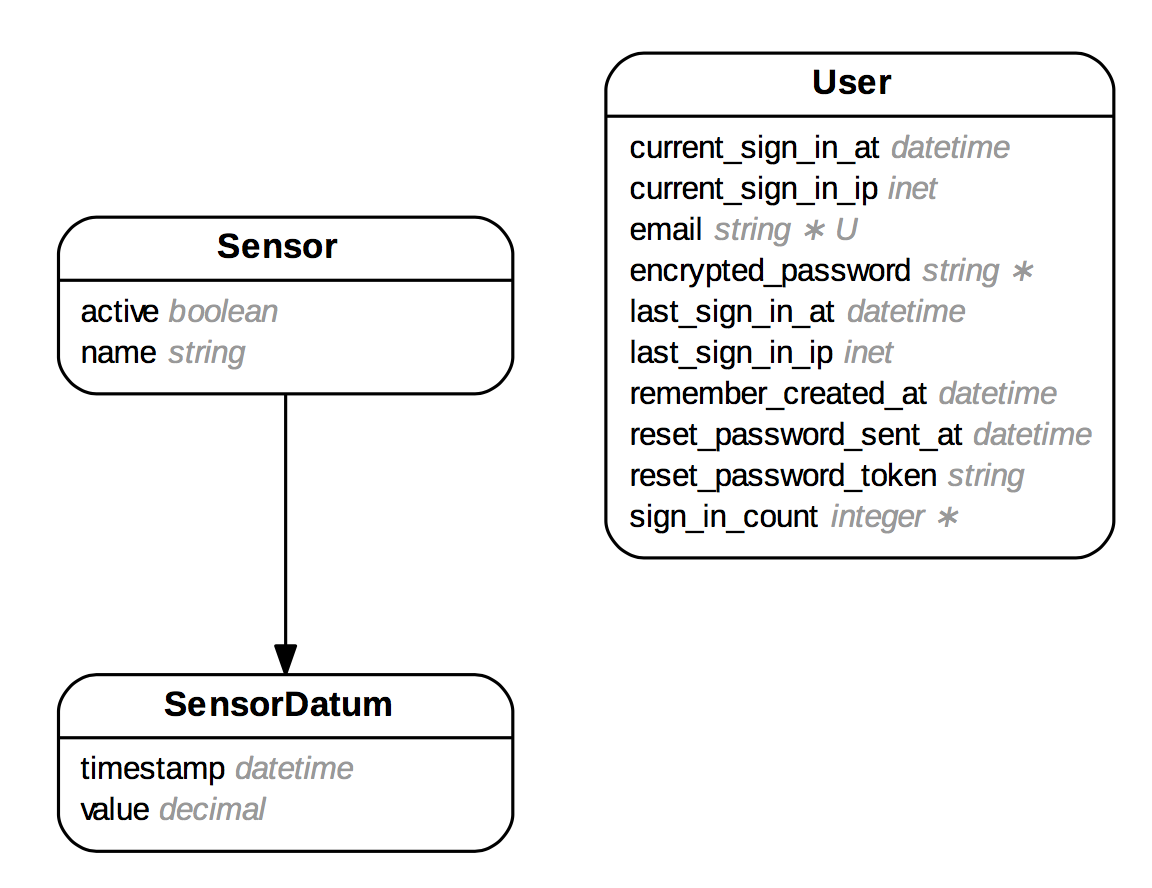
\includegraphics[width=\linewidth]{images/diagram_erd}
  \caption{Diagram ERD bazy danych.}
  \label{fig:diagram_erd}
\end{figure}
\newpage
\section{Ruby on Rails}
Framework \emph{Ruby on Rails} domyślnie korzysta z architektury \emph{MVC}. Aby nie łamać zasady \emph{Convention over Configuration}, zdecydowano się stworzyć aplikację zgodną z ideą frameworka, czyli w tej właśnie architekturze.

\subsection{Modele}
Aplikacja posiada 3 modele: \emph{User}, \emph{TemperatureSensor} oraz \emph{TemperatureSensorDatum}. Dodatkowo, korzystając z mechanizmu \emph{STI} (ang. \emph{Single Table Inheritation}), istnieją dwa modele abstrakcyjne \emph{Sensor} oraz \emph{SensorDatum}, które są bazą dla różnych typów sensorów oraz danych zbierane przez owe sensory. Na listingach \ref{lst:rails_sensor} oraz \ref{lst:rails_temp_sensor} przedstawiony jest przykład implementacji \emph{STI}, czyli abstrakcyjny model sensora oraz dziedziczący po nim model \emph{TemperatureSensor}.
\newpage

\begin{lstlisting}[caption={Abstrakcyjny model sensora w Ruby on Rails.},label={lst:rails_sensor},language=Ruby]
class Sensor < ApplicationRecord
end
\end{lstlisting}

\begin{lstlisting}[caption={Model sensora temperatury w Ruby on Rails.},label={lst:rails_temp_sensor},language=Ruby]
class TemperatureSensor < Sensor
  has_many :temperature_sensor_data
end
\end{lstlisting}

Łatwo zauważyć, że abstrakcyjny model jest praktycznie pusty. Jedyną ważną informacją jest dziedziczenie po klasie \emph{ApplicationRecord}, po której musi dziedziczyć każdy model. Natomiast w klasie \emph{TemperatureSensor} zdefiniowana jest relacja jeden do wielu z danymi sensora.

\subsection{Kontrolery}


\subsection{Widoki}


\section{Phoenix}
\subsection{Modele}

\subsection{Kontrolery}

\subsection{Widoki}


\section{Express}
\subsection{Modele}

\subsection{Kontrolery}

\subsection{Widoki}
